\documentclass[12pt]{article}
\title{Temperature Changes in Florida over Sucessive years}
\author{Rachel Bates}
\date{24.10.18}
\usepackage{graphicx}

\begin{document}
  \maketitle

  \begin{abstract}
  This paper looks at how to calculate a p-value for temperature changes between sucessive years, using data from Florida as an example.  
  \end{abstract}

  \section{Methods}
  The temperatures from the sample set were randomly jumbled using R's sample function. A correlation coefficient was then determined for sucessive values on this list. This was done 10000 times to produce a distribution of values independant of the effect of year.

  \section{Results}
  The correlation coefficient for the correctly ordered data was 0.306 (3 s.f.)
  The sampled correlation coefficients ranged from -0.370 to 0.416, with a median of -0.010. Only 5 values were larger than the real data, giving an approximate p-value for the real data of $< 0.001$. 
  See Figure 1. for a graphical representation of the real value in relation to distribution of sampled values.

  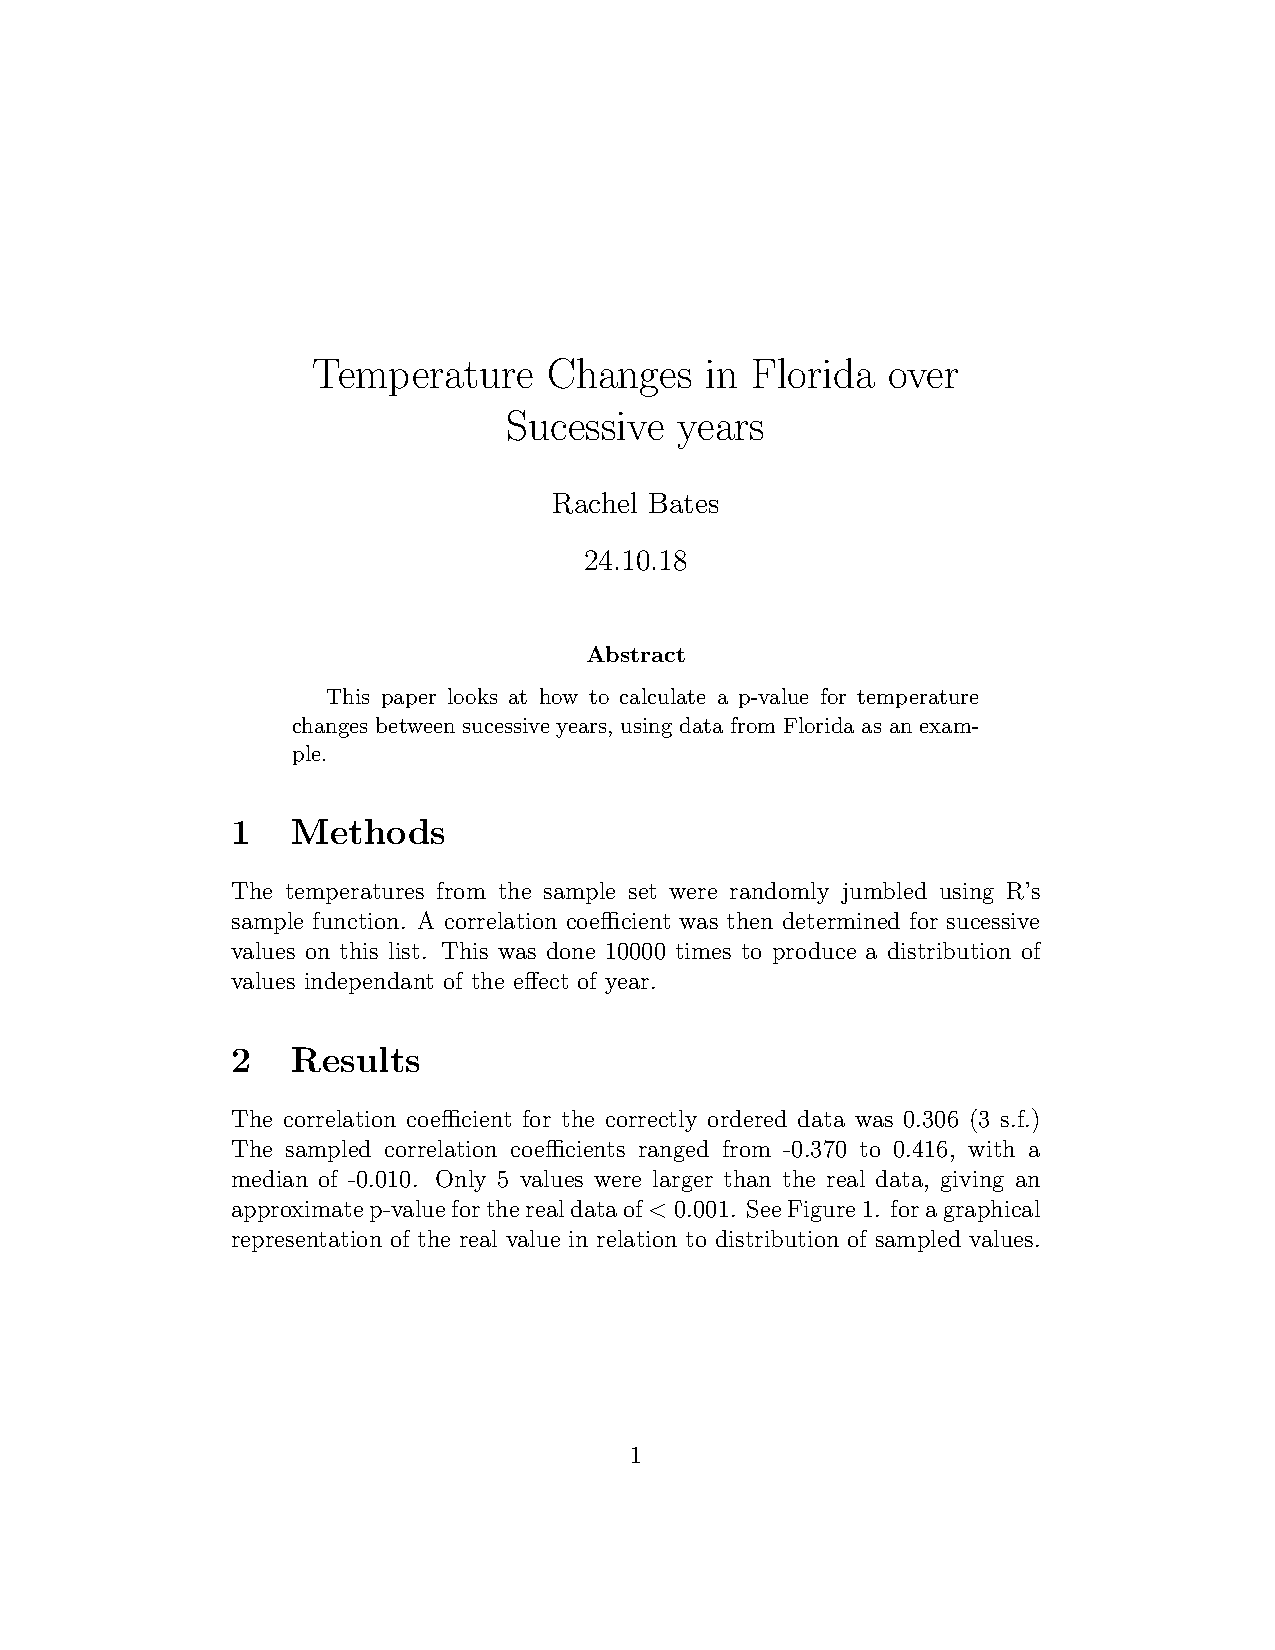
\includegraphics[width=0.98\textwidth]{../Output/TAutoCorr}

  Figure 1. Distribution of n=10000 sampled correlation coefficients using temperature data from sucessive years in Florida. The correlation coefficient from the non-scrambled data is included as a line.

\end{document}